\documentclass[10pt,a4paper,twocolumn]{article}
\usepackage{graphicx}
\usepackage{color}
\usepackage{hyperref}
\begin{document}

\title{Experiment of training Full Ternary Weights Network(FTWN) with darknet YOLO}
\author{Kenji Ogura}
\date{}
\maketitle

\section{Abstract}
Generally ternarizing weights of neural network model requires retraining after ternarization of weights.
To reduce accuracy damage by ternarization I propose the staged retraining method(SRM) for full ternary weights network(FTWN).
At SRM retraining and ternarizing pair consist of 4 pairs of Ternarizing and retraining to avoid local minumum problem.
SRM widens ternarizing layers from full precision until FTWN step by step.
To confirm effect of SRM at experiment I customized darknet framework to support weights ternarizing in convolutional layer and integrated training algorithm in it.
I trained yolov2 and yolov3 models on customized darknet framework with VOC dataset 2012 and 2007 and obtained mAP as results.
Full ternarized yolov2 with SRM performs 73.82\% mAP against full precision's 76.85\% mAP.
Full ternarized yolov3 with SRM performs 71.26\% mAP against full precision's 75.54\% mAP.

\section{Introduction}

Some quantinization methods for model weights are proposed such as FP16, bfloat, fixed point 16bits, 8bit, ternary 2bits and XNor 1bit.
Generally the inference task using full ternary weights -1,0,+1 with scaling factor Wl is considered as low accuracy than full precision weights.
However for low power device such as mobile phone small weights will be efficient one of choices and 2bits ternary weights representaion may be x16 smaller than 32bit floating point.
I consider that quatinization of weights requires retraining after quantinization.
In this paper I propose Staged Retrainiing Method(SRM) for full ternary weights network and show the result as mAP.

\section{Related works}

I refer to papers which denote efficiency of quantinization about XNOR and Ternary weights.
\begin{itemize}
\item
 Training algorithm : "Alorithm 1" in "XNOR-Net: ImageNet Classification Using BinaryConvolutional Neural Networks"\cite{Rastegari2015XNORNetIC}
\item
 Conversion system to Ternarize weights with scale factor Wl from full precision weigts : "2.2 Approximated solution with threshold-based ternary function" in "Ternary weight networks"\cite{Li2016TernaryWN}
\end{itemize}

I implement above Training algorithm and Conversion system into \href{https://github.com/pjreddie/darknet}{darknet code} for this experiment.

\section{Staged Retraining Method}

I propose the staged retraining method(SRM) for full ternarization of model weights suppressing accuracy damage.
To avoid local minimun problem during retraining ternarized model splitting retraining into some steps is important.
In experiment SRM generates full ternarized weights for yolov2-voc\cite{redmon2016yolo9000}, yolov3-voc\cite{yolov3} by splitting a training step into 4 stages.
Roughly staging plan is below,

\begin{itemize}
\item Stage-0 : few layers without around of detector are ternarized(M0)
\item Stage-1 : 40\% of all layers are ternarized(M1)
\item Stage-2 : 90\% of all layers are ternarized(M2)
\item Stage-3 : full ternarized(M3)
\end{itemize}

Each stages from M1 to M3 import weights from previous stage, such as stage-2 weights from stage-1.
However stage-0 M0 imports usual full precision weights.
Figure.1 shows staging for yolov2-voc.cfg into 4 training stages and Figure.2 for yolov3-voc.cfg.
On each figures 'F' denote full precision layer and 'T' denotes ternarized layer.
To estimate SRM I implement ternary keyword for each convolution layer in cfg file like 'ternary=1' and I also implement ternarizing weights function including conversion system\cite{Li2016TernaryWN} and memory area saving for the ternarized weights in \href{https://pjreddie.com/darknet/yolo}{darknet framework}.

\begin{figure}
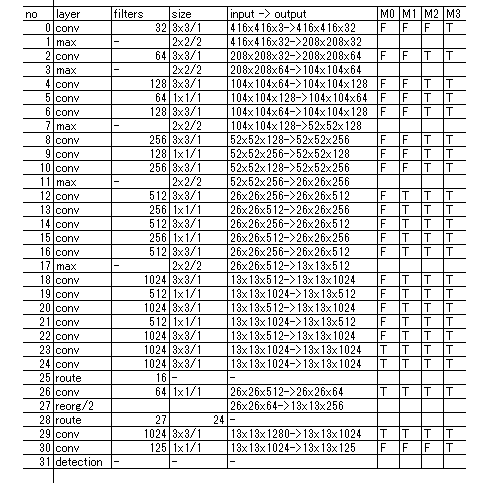
\includegraphics[width=8cm]{YOLOV2VOCSTAGES.PNG}
\caption{Staging for yolov2-voc.cfg}
\end{figure}

\begin{figure}
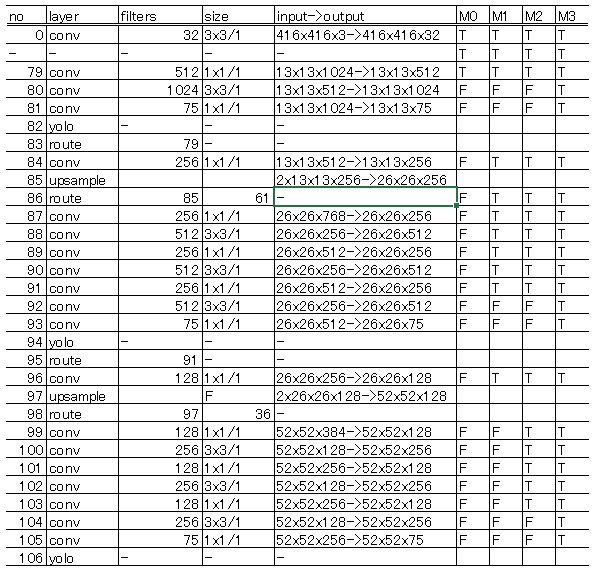
\includegraphics[width=8cm]{YOLOV3VOCSTAGES.PNG}
\caption{Staging for yolov3-voc.cfg}
\end{figure}

I retrained yolov2-voc.cfg on 4 jobs, and checked each loss curves on Excell graph.
And I use \href{https://github.com/AlexeyAB/darknet}{AlexeyAB darknet} to get mAP of experiments.

\section{Result of Experiment}

Tables denote the result of retraining with SRM.
VOC 2012, 2007 Dataset is used with training and VOC 2007 for estimation of mAP.

\begin{table}[htbp]
 \centering
 \begin{tabular}{c|c|c|l}
  Stage & mAP & IOU & comments \\ \hline\hline
  -        & 76.85 & 54.67 & official weights \\ \hline
  M0       & 77.09 & 57.04 & -                \\ \hline
  M1       & 76.44 & 56.18 & -                \\ \hline
  M2       & 75.06 & 57.71 & -                \\ \hline
  M3       & 73.82 & 54.90 & full ternary     \\ \hline\hline
 \end{tabular}
 \caption{result regard to yolov2}
 \label{tb:yolov2}
\end{table}

In Table.1 Iteration 41000(2000/class), steps x0.1 80\% 90\%, lr=0.001 at all stages
official weights denotes full precision weights downloaded from \href{https://pjreddie.com/darknet/yolov2}{darknet website for yolov2}.

\begin{table}[htbp]
 \centering
 \begin{tabular}{c|c|c|l}
  Stage & mAP & IOU & comments \\ \hline\hline
  -        & 75.54 & 62.78 & darknet53.conv.75 \\ \hline
  M0       & 75.02 & 63.04 & -                \\ \hline
  M1       & 73.69 & 63.75 & -                \\ \hline
  M2       & 73.76 & 63.54 & -                \\ \hline
  M3       & 71.26 & 61.61 & full ternary     \\ \hline\hline
 \end{tabular}
 \caption{result regard to yolov3}
 \label{tb:yolov3}
\end{table}

In Table.2 Iteration 100400(5000/class), steps x0.1 80\% 90\%, lr=0.001 at M0 and M1
Iteration 60400(3000/class), steps x0.1 80\% 90\%, lr=0.001 at M2 and M3.
darknet53.conv.75 denotes full precision weights downloaded from \href{https://pjreddie.com/darknet/yolo}{darknet website} and partialized until 75 layers.

\section{Conclusion}

If your applications using object detection task requires speed but not accuracy you can use full ternary weights network.
To get efficient ternary weights you can use staged retraining method and generally full ternary weights is x16 smaller than fp32 representation.
In experimet full ternary weights network via yolov2 or yolov3 perform accuracy within 4.5\% mAP drops against full precision network.

\begin{thebibliography}{1}

\bibitem{Li2016TernaryWN}
Fengfu Li and Bin Liu.
\newblock Ternary weight networks.
\newblock {\em ArXiv}, abs/1605.04711, 2016.

\bibitem{Xu2018TrainingAB}
Jiaolong Xu, Peng Wang, Haishun Yang, and Antonio.Lpez.
\newblock Training a binary weight object detector by knowledge transfer for
  autonomous driving.
\newblock {\em 2019 International Conference on Robotics and Automation
  (ICRA)}, pages 2379--2384, 2018.

\bibitem{Rastegari2015XNORNetIC}
Mohammad Rastegari, Vicente Ordonez, Joseph Redmon, and Ali Farhadi.
\newblock Xnor-net: Imagenet classification using binary convolutional neural
  networks.
\newblock {\em ArXiv}, abs/1603.05279, 2016.

\bibitem{redmon2016yolo9000}
Joseph Redmon and Ali Farhadi.
\newblock Yolo9000: Better, faster, stronger.
\newblock {\em arXiv preprint arXiv:1612.08242}, 2016.

\bibitem{yolov3}
Joseph Redmon and Ali Farhadi.
\newblock Yolov3: An incremental improvement.
\newblock {\em arXiv}, 2018.

\end{thebibliography}

\end{document}
